\documentclass[aspectratio=169,10pt]{beamer}
\usetheme{Madrid}
\usecolortheme{dolphin}
\usepackage[utf8]{inputenc}
\usepackage[T1]{fontenc}
\usepackage[spanish]{babel}
\usepackage{graphicx,booktabs,tabularx}
\newcommand{\parencite}[1]{\textsuperscript{[#1]}}
\renewcommand{\cite}[1]{\textsuperscript{[#1]}}
\title{Netflix: RPC, gRPC y RMI en un sistema distribuido real}
\subtitle{GA-SUM-02 / EXP-1}
\author{Jordan Loor \and Steven Pozo \and Luis Quintero \and Leonel Zambrano}
\institute{UTEQ -- Aplicaciones Distribuidas}
\date{21 de noviembre de 2026}
\setbeamertemplate{navigation symbols}{}
\begin{document}
\begin{frame}\titlepage\end{frame}

\section{Presentación de Netflix}

\begin{frame}{Netflix: plataforma de entretenimiento global}
    \begin{itemize}
        \item Plataforma de series, películas, videojuegos y programación en directo.
        \item Servicio disponible internacionalmente.
        \item Operaciones de streaming organizadas en cuatro regiones.
    \end{itemize}

    \vspace{0.3cm}

    \begin{block}{Resultados de 2025}
        \centering
        {\Large 45.183 millones USD}

        Ingresos anuales

        \vspace{0.15cm}
        \textbf{16\%} de crecimiento respecto a 2024.
    \end{block}

    \parencite{netflix2025annual}
\end{frame}


\section{Transparencias de distribución}

\begin{frame}{Transparencia de ubicación y replicación}
    \begin{columns}[T]
        \column{0.48\textwidth}
        \textbf{Ubicación (Eureka)}

        \begin{itemize}
            \item Nombres virtuales (VIP).
            \item Descubrimiento de servicios.
            \item Localización de instancias.
        \end{itemize}

        \column{0.48\textwidth}
        \textbf{Replicación (Ribbon)}

        \begin{itemize}
            \item Varias instancias.
            \item Balanceo del lado del cliente.
            \item Distribución de solicitudes.
        \end{itemize}
    \end{columns}

    \vspace{0.3cm}
    \centering
    \textit{El consumidor no necesita seleccionar manualmente cada máquina.}

    \parencite{vroom2023mesh}
\end{frame}


\begin{frame}{Comparación de comunicación entre microservicios}

    \begin{itemize}
        \item Estudio de Niswar et al. (2024).
        \item Comparación de REST, GraphQL y gRPC.
        \item Caso de estudio: sistema SISTER.
    \end{itemize}

    \vspace{0.3cm}

    \begin{block}{Resultados con 100 solicitudes}
        \begin{itemize}
            \item Datos planos: gRPC obtuvo el menor tiempo
            de respuesta (233,84 ms).
            \item Datos anidados: REST obtuvo el menor
            tiempo (5.201,39 ms).
        \end{itemize}
    \end{block}

    \centering
    \textit{La mejor alternativa depende del tipo de consulta.}

    \parencite{niswar2024grpc}

\end{frame}


\begin{frame}{Transparencia de acceso y limitaciones}

    \textbf{Acceso (Envoy)}

    \begin{itemize}
        \item Proxy local para facilitar la comunicación.
        \item Descubrimiento y conexión entre servicios.
        \item Menos lógica de comunicación en las aplicaciones.
    \end{itemize}

    \vspace{0.2cm}

    \textbf{Limitaciones}

    \begin{itemize}
        \item Eureka puede conservar información desactualizada.
        \item La primera solicitud puede añadir latencia.
        \item Los fallos de red siguen siendo posibles.
    \end{itemize}

    \parencite{vroom2023mesh}
\end{frame}


\section{Lecciones para el PFC}

\begin{frame}{Lecciones para nuestro PFC}

    \begin{itemize}
        \item Definir contratos claros entre servicios.
        \item Elegir mecanismos de comunicación adecuados.
        \item Gestionar errores y considerar la latencia.
        \item Evaluar los costos de una arquitectura de microservicios.
    \end{itemize}

    \vspace{0.3cm}

    \centering
    \textbf{La comunicación entre servicios debe ser clara y confiable.}

    \parencite{henriquez2025netflix}
\end{frame}

% Diapositivas de Steven Pozo - avance Día 1

\begin{frame}{Arquitectura: vista respaldada por evidencia}
  \begin{columns}[T]
    \begin{column}{0.62\textwidth}
      \centering
      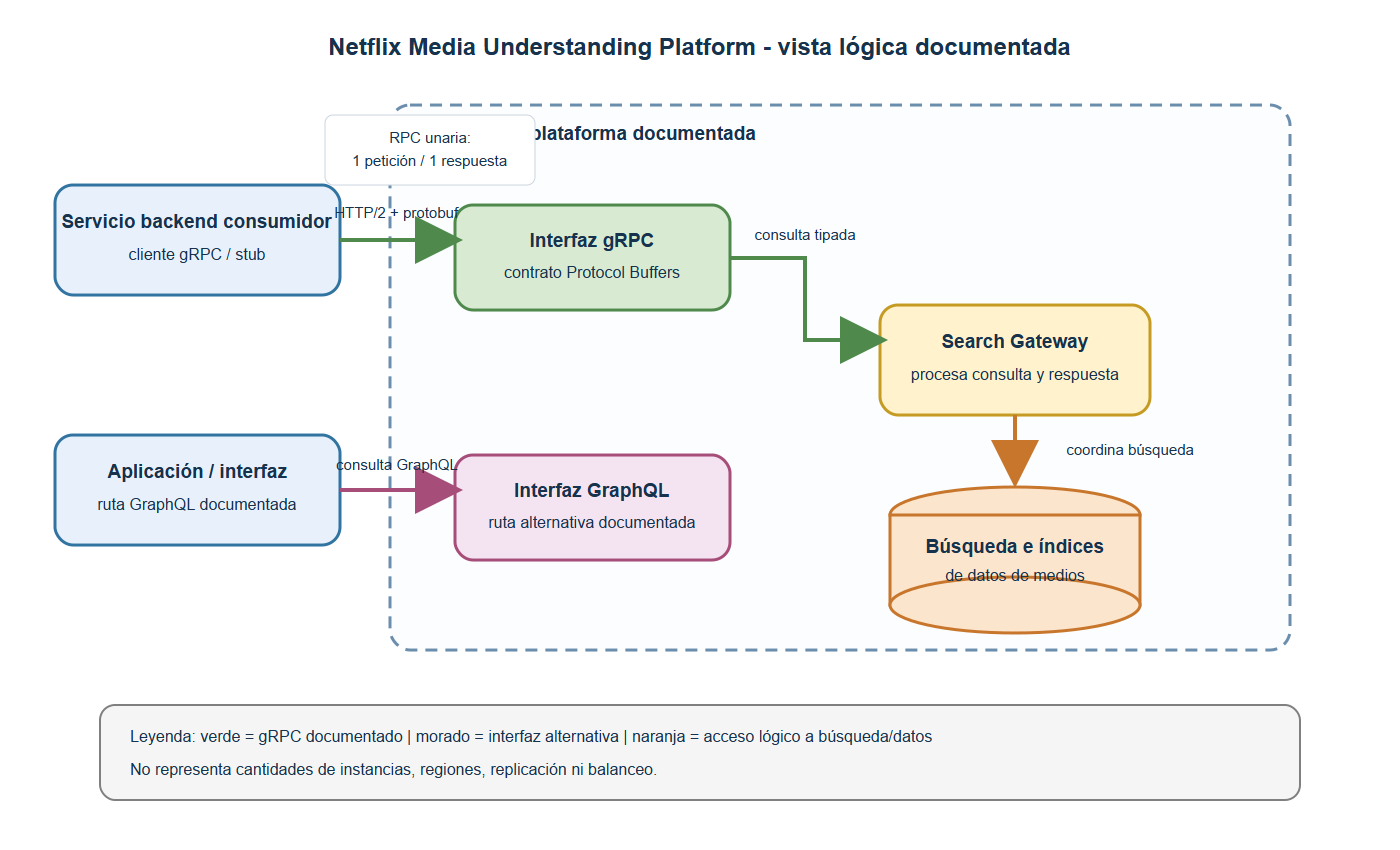
\includegraphics[width=\linewidth]{figuras/arquitectura.png}
    \end{column}
    \begin{column}{0.36\textwidth}
      \begin{itemize}
        \item Caso: Media Understanding Platform
        \item Cliente gRPC: servicio backend consumidor
        \item La aplicación final usa la ruta GraphQL mostrada
        \item Search Gateway coordina consultas
        \item Vista lógica, no topología física completa
      \end{itemize}
    \end{column}
  \end{columns}
  \vfill
  {\tiny Fuente: Netflix Technology Blog (2023), ``Building a Media
  Understanding Platform for ML Innovations''.}
\end{frame}

\begin{frame}{Modelo cliente-servidor y RPC unaria}
  \begin{block}{Una invocación remota}
    Backend cliente / stub $\rightarrow$ una petición protobuf $\rightarrow$ servicio
    gRPC $\rightarrow$ una respuesta o estado.
  \end{block}
  \begin{itemize}
    \item Contrato de servicio definido con Protocol Buffers.
    \item Transporte habitual de gRPC: HTTP/2.
    \item Generación de clientes para varios lenguajes.
    \item La red sigue siendo visible: latencia, deadline y errores.
  \end{itemize}
  \begin{alertblock}{Límite de la afirmación}
    gRPC no garantiza por sí solo replicación, disponibilidad, consistencia ni
    recuperación ante fallos.
  \end{alertblock}
  \vfill
  {\tiny Fuentes: documentación oficial de gRPC; caso de estudio CNCF/Netflix.}
\end{frame}

\begin{frame}{Secuencia de una RPC unaria}
  \begin{enumerate}
    \item El cliente invoca un método del \textbf{stub}.
    \item gRPC serializa una petición con \textbf{Protocol Buffers}.
    \item El servidor ejecuta la operación solicitada.
    \item Regresa una respuesta y un estado, o un error.
  \end{enumerate}
  \begin{block}{Regla para recordarla}
    Invocar $\rightarrow$ serializar $\rightarrow$ ejecutar $\rightarrow$ responder.
  \end{block}
  \begin{alertblock}{No es una función local}
    La llamada cruza la red: puede tener latencia, superar su plazo o fallar.
  \end{alertblock}
  \vfill
  {\tiny Fuente: documentación oficial de gRPC, ``Core concepts, architecture
  and lifecycle''.}
\end{frame}

\section{CAP, PACELC y comparación}

\begin{frame}{CAP/PACELC: no etiquetamos a Netflix completo}
\begin{block}{Caso delimitado: EVCache para datos no críticos}
\textbf{Partición:} operación local disponible; replicación remota asíncrona.
\quad $\Rightarrow$ aproximación AP para este caso.

\textbf{Sin partición:} lectura local de baja latencia; posible diferencia
temporal entre regiones. \quad $\Rightarrow$ aproximación EL.
\end{block}
\begin{alertblock}{Límite}
gRPC no decide CAP. Otros almacenes de Netflix usan cuórum y garantías de
lectura después de escritura.
\end{alertblock}
{\footnotesize Fuentes: Netflix Technology Blog \cite{netflix-evcache,netflix-media-db}.}
\end{frame}

\begin{frame}{Netflix frente a infraestructura de video de YouTube}
\small
\begin{tabularx}{\linewidth}{@{}p{2.1cm}XX@{}}
\toprule
 & \textbf{Netflix} & \textbf{YouTube/Google} \\
\midrule
Arquitectura & Microservicios, cachés y almacenes distribuidos & Software
distribuido y aceleradores VCU \\
Comunicación & gRPC documentado entre backends & La fuente no identifica un RPC
concreto \\
Trade-off & Latencia frente a consistencia en EVCache & Eficiencia frente a
especialización de hardware \\
\bottomrule
\end{tabularx}
\medskip
Google reportó entre \textbf{20 y 33 veces} mayor eficiencia frente a su
plataforma previa \cite{google-vcu}.
\end{frame}

% Cargar este archivo una vez. Invocar cada bloque en su turno del programa.
\newcommand{\LeonelComunicacion}{
\begin{frame}{Una consulta puede devolver una página parcial}
\texttt{GetItems} solicita registros a la capa de datos de Netflix.
\begin{enumerate}
\item El servidor controla el tiempo que lleva la consulta.
\item Si peligra el objetivo de latencia, devuelve los datos reunidos y un token.
\item El cliente puede usar el token para pedir la página siguiente si queda tiempo.
\end{enumerate}
{\footnotesize Capa clave-valor de Netflix y plazos de gRPC \cite{leonel-kv,fallos-grpc}.}
\end{frame}}

\newcommand{\LeonelFallos}{
\begin{frame}{PlayAPI protegió las peticiones del usuario}
Después de una caída, Android multiplicó por \textbf{12} sus solicitudes de precarga por segundo.
\medskip

\begin{tabular}{@{}lr@{}}
\textbf{Tipo de petición} & \textbf{Disponibilidad}\\[3pt]
Precarga automática & mínimo del 20\,\%\\
Iniciada por el usuario & superior al 99,4\,\%\\
\end{tabular}
\medskip

El servicio descartó primero las precargas \cite{fallos-netflix}.
\end{frame}

\begin{frame}{Paul vs.\ Tyson: pausas durante la transmisión}
15 de noviembre de 2024 \hfill Más de 60 millones de hogares \cite{fallos-temple}
\medskip
\begin{description}
\item[Impacto] Miles de espectadores reportaron pausas.
\item[Indicio] Las pruebas apuntaron a congestión en los servidores de entrega durante el pico de demanda.
\item[Mitigación] Muchas pruebas recuperaron el video al reconectar con una tasa de bits menor.
\end{description}
{\footnotesize Diagnóstico externo de ThousandEyes \cite{fallos-thousandeyes}.}
\end{frame}}

\newcommand{\LeonelCierre}{
\begin{frame}{¿Qué acción protegeríamos en el PFC?}
\begin{enumerate}
\item Elegir una acción esencial y una tarea secundaria.
\item Aumentar la carga y posponer parte del trabajo secundario.
\item Comparar qué porcentaje de cada tipo de petición termina a tiempo.
\end{enumerate}
\end{frame}}


\LeonelComunicacion
\LeonelFallos
\LeonelCierre
\begin{frame}{Conclusiones}
\begin{itemize}
\item gRPC ofrece contratos tipados, pero no elimina latencia ni fallos de red.
\item CAP/PACELC debe analizarse por dato y operación, no por empresa o protocolo.
\item La resiliencia requiere priorización, plazos y decisiones ante sobrecarga.
\item RMI conserva utilidad en entornos Java homogéneos; no se atribuye a Netflix.
\end{itemize}
\end{frame}
\begin{frame}{Referencias principales}
\tiny
\begin{itemize}
\item Netflix Technology Blog (2023), Service Mesh con descubrimiento bajo demanda.
\item Netflix Technology Blog (2024), capa de datos clave--valor y load shedding.
\item Netflix Technology Blog, Media Understanding Platform y EVCache global.
\item gRPC, documentación oficial de deadlines y llamadas unarias.
\item Niswar et al. (2024), DOI: 10.24425/ijet.2024.149562.
\item Henríquez et al. (2025), DOI: 10.15665/rp.v23i1.3683.
\item Ranganathan et al. (2021), DOI: 10.1145/3445814.3446723.
\end{itemize}
\end{frame}
\end{document}
